% This is LLNCS.DEM the demonstration file of
% the LaTeX macro package from Springer-Verlag
% for Lecture Notes in Computer Science,
% version 2.4 for LaTeX2e as of 16. April 2010
%
\documentclass[12pt,article,oneside]{memoir}
%
\usepackage{tikz}
\usepackage{geometry}
\usepackage{multirow}
\usepackage{hyperref}
\usepackage{breakurl}
\usepackage{float}
\usepackage{makeidx}  % allows for indexgeneration
\usepackage[sectionbib,numbers,sort&compress]{natbib}
\usepackage{footnote}
\usepackage{graphicx}
\usepackage{wrapfig}
\usepackage{listings}
%\usepackage{url}
%
\geometry{
	a4paper,
	left=1.25in,
	right=1.25in,
	top=1.25in,
	bottom=1.25in
}


%----------------------------------------------------------------------------
%   CUSTOM COMMANDS
%----------------------------------------------------------------------------
% Command for "key words" (in this paper, the features of the dataset)
\newcommand{\key}[1]{#1}
% Command for R function names
\newcommand{\func}[1]{\texttt{\color{red} #1}}

\counterwithout{section}{chapter} % Start section number at 1, 2, .. instead of 0.1, 0.2, ...
\newcommand{\specialcell}[2][c]{%
	\begin{tabular}[#1]{@{}c@{}}#2\end{tabular}}

\usepackage{graphicx} %remove demo in your file.
\usepackage[export]{adjustbox}
\usepackage{letltxmacro}


% Set font family to sans-serif
\renewcommand{\familydefault}{\sfdefault}

\begin{document}
%
%

\pagestyle{headings}  % switches on printing of running heads
%\mainmatter              % start of the contributions
\title{Assignment \#2 for STAT 5703W}
%
%\titlerunning{Challenges in Representation Learning}  % abbreviated title (for running head)
%                                     also used for the TOC unless
%                                     \toctitle is used
%
\author{Philippe Paradis\\\medskip Carleton University\\ \texttt{philippe.paradis@gmail.com}}
%
%
%\institute{Carleton University\\
%\email{philippe.paradis@carleton.ca}}

\setcounter{tocdepth}{4}
\setcounter{secnumdepth}{4}
\maketitle              % typeset the title of the contribution

\begin{abstract}
Assignment \#2 in STAT5703W.
%\keywords{R, data visualization}
\end{abstract}
%

\tableofcontents

\section{Question 1}

\subsection{Principal Component Analysis for Handwritten Digits}
The handwritten digits dataset is a series of images stored in text format. Each row is a sequence of 256 floating point values ranging between $-1.0$ and $1.0$ and representing a pixel intensity value in a $16 \times 16$ grayscale image. The quantity of training examples varies by digit, as you can see from the following table.
% latex table generated in R 3.1.2 by xtable 1.7-4 package
% Tue Mar 10 06:26:10 2015
\begin{table}[H]
	\centering
	\begin{tabular}{rrrrrrrrrrr}
		\hline
		\textbf{Digit} & 0 & 1 & 2 & 3 & 4 & 5 & 6 & 7 & 8 & 9 \\ 
		\hline
		\textbf{Training examples} & 1194 & 1005 & 731 & 658 & 652 & 556 & 664 & 645 & 542 & 644 \\ 
		\textbf{Features} & 256 & 256 & 256 & 256 & 256 & 256 & 256 & 256 & 256 & 256 \\ 
		\hline
	\end{tabular}
	\label{table:dataset}
\end{table}
\emph{Principal Component Analysis} is a dimensionality reduction technique. We expect dimensionality reduction to be useful for the handwritten digits dataset, because it has 256 features or dimensions, yet the underlying \emph{intrinsic dimension} (in the informal sense of the term) of the space of handwritten digits should be much lower. 

We run \func{prcomp} in R on each digit's training dataset and produce a bar plot in Figure\ref{fig:digits-pca} of the variance associated with the first few principal components. 

\begin{figure}[htb]
\adjincludegraphics[width=1.2\textwidth, center]{figures/digits-pca.pdf}
\caption{Bar plots of variance explained by the top principal components obtained from running PCA on each handwritten digit training dataset.}
\label{fig:digits-pca}
\end{figure}

\subsection{Variance Explained by the Principal Components}

We investigate how many principal components are required in order to explain at least 95\% of the variance of a dataset. This can be computed easily from the results of \func{prcomp}. We compute this in the function \func{how.many.pcs.for.variance(0.9)} (see Appendix) and obtain the following table.
% latex table generated in R 3.1.2 by xtable 1.7-4 package
% Sun Mar 15 03:45:22 2015
\begin{table}[ht]
\centering
\begin{tabular}{rrrrrrrrrrr}
  \hline
  \textbf{Digit}            &   0 &   1 &   2 &   3 &   4 &   5 &   6 &   7 &   8 &   9 \\ 
  \textbf{\# of Components} &  36 &   2 &  58 &  47 &  42 &  49 &  30 &  22 &  45 &  24 \\ 
   \hline
\end{tabular}
\caption{Number of top principal components required to account for at least 95\% of the digit dataset variance}
\end{table}
Observe that the ``simple'' digit 1 requires very few principal components to account for the variance, compared to the other digits. This makes sense, because it is the simplest digit and most of its variance is accounted for by its width.

\subsection{What Does a Principal Component Look Like?}

Let us recall how \func{prcomp} works. If $V$ is the input training set, then the output of \func{prcomp} will contain the orthogonal transformation \func{prcomp(V)\$rotation}, which we denote as $W$, and the transformed set of vectors \func{prcomp(V)\$x}, which we also denote as $X$, such that
	\[X = VW.\]
Now, since $W$ is an orthogonal matrix, then the transpose of $W$ is the inverse of $W$. As such, if we want to know what the principal components look like, we can multiply by $W^{-1}$ and we get
\[V = X W^{-1} = X W^t\]
From this, we deduce that $PC1$ is equal to $e_1 W^t$, i.e. $PC1$ is the first row of $W^t$. Similarly, $PC2$ is the second row of $W^t$, and so on.

Therefore, we will be able to inspect the principal components by plotting the first few rows of \func{t(prcomp(V)\$rotation)}. For example, let us look at the top 40 principal components of the digit $0$.
\begin{figure}[H]
	\adjincludegraphics[width=0.98\textwidth, center]{figures/top-pcs-digit-0}
	\caption{The top 40 principal components of digit 0. The image in the top-left corner is $PC1$ and it continues in increasing order from left to right and then from top to bottom.}
	\label{fig:top-pcs-digit-0}
\end{figure}

Those images tell us where the greatest variation in our data lie. For example, the first principal component indicate a high variance in the width of the digit. We illustrate this by graphing an image of the average values over the training dataset for this digit and then adding a multiple of the first principal component ($PC1$).

\begin{figure}[H]
	\adjincludegraphics[width=0.98\textwidth, center]{figures/pc-2}
	\caption{Variation along $PC2$}
	\label{fig:pc-2}
\end{figure}

As we can see from Figure~\label{fig:pc-2}, $PC2$ measures the width of the digits 0, 1, 3, 6, 7, 8 and 9. On the other hand, it would appear to measure the height of the digit 2. The interpretation of what feature is measured for the digit 4 is less clear, but it seems to be the intensity of its upper-left segment. Finally, $PC2$ appears to measure the ratio between the width of the top and bottom for the digit 5.

This corresponds to what was expected when looking at Figure~\label{fig:top-pcs-digit-0}.

\subsection{PCA Reconstruction}

In this section we investigate the properties of PCA, specifically for the purpose of \emph{dimensionality reduction} and as such, we ignore the other numerous uses of PCA. Let us assume that we would like to reduce the number of dimensions from 256 to some smaller number, say $d$.

A handwritten digit is a vector $v$ of length $256$ where the entries represent pixel intensity values. After applying PCA, each handwritten digit becomes a vector $x$ of length $256$ where the entries represent the coefficients of $PC1, \ldots, PC256$.

PCA works by producing an orthogonal matrix $W$, which gives the translation $x = Wv$. Since any orthogonal matrix is invertible, it is clear that no information is lost by applying PCA as long as all the principal components are preserved.

At this point, data dimensionality reduction can be carried out. Each vector $x$ is truncated to a vector $\hat{x}$ of length $d$. That is, only the coefficients $PC1,$ $\ldots,$ $PCd$ of the top $d$ principal components are preserved or saved, whereas the coefficients $PC(d+1),$ $\ldots,$ $PC256$ are discarded or lost.

This naturally lead to the following idea. What if we multiply $\hat{x}$ by $W^t$ to recover an approximation of $v$? This would tell us more information about exactly the nature of the information lost or preserved during PCA dimensionality reduction. To study this, we looked at at reconstruction of the digit $0$ using different amount of top principal components in Figure~\ref{fig:recreate-gradual-digit-0}.

\begin{figure}[H]
	\adjincludegraphics[width=0.98\textwidth, center]{figures/recreate-gradual-digit-0}
	\caption{The first column indicates how many top principal components were used to recreate the first 12 training examples for the digit 0.}
	\label{fig:recreate-gradual-digit-0}
\end{figure}

As we can see from Figure~\ref{fig:recreate-gradual-digit-0}:
\begin{itemize}
	\item Using 30 principal components or less, this reconstruction is very good at smoothing out the noise.
	\item Using between 5 and 30 components, the general size and shape of the digits is preserved, but the small irrelevant details are lost.
	\item Using less than 5 components, the digits are very similar to each other and quite different from the original version.
\end{itemize}

\subsection{What Next?}

In a future investigation, we would like to combine all the handwritten digit datasets into one and apply PCA to that set. 

Moreover, we would like a more precise answer to the following two questions:
 \begin{enumerate}
 	\item What characterizes the data that is saved?
 	\item What characterizes the data that is lost?
 \end{enumerate}
 It is the author's opinion that question 2 is particularly important. For example, we would like to know: Is the lost data simply noise? When is it not appropriate to use PCA?

%Notes to self:
%* Keep in mind that the point of PCA is to reduce dimension
%* We just drop the "extra" data
%* Then, it's interesting to note what happens when we try to reconstruct the
%original data from the PCA data
%* It's also interesting to note what are some properties of the PCA data
%** For example, what characterizes the data we kept?
%** What characterizes the data we dropped? Is it just noise, or something else? (I THINK
%THIS MIGHT BE THE MOST IMPORTANT QUESTION)
%** What are the pros and cons of using PCA.
%** When should we use PCA?

% TODO: Do some analysis of properties of PCA when its ran on the combined training sets

\subsection{Independent Component Analysis for Handwritten Digits}

For Independent Component Analysis, we combine the training datasets of all digits into one. Then, we use the function \func{fastICA} with \func{n.comp = 40} components. Moreover, because the classes are not balanced, we restricted ourselves to the first 400 images in each digit's training dataset. That is, we built a balanced combined training set of 4000 images.q The resulting 40 independent components or ''sources`` are displayed in Figure~\ref{fig:ica-components}.
\begin{figure}[H]
	\adjincludegraphics[width=0.98\textwidth, center]{figures/ica-components}
	\caption{The sources -- or independent components -- of the handwritten digits training sets for \func{n.comp = 40}.}
	\label{fig:ica-components}
\end{figure}

Notice that the sources in Figure~\ref{fig:ica-components} have almost no overlap. Moreover, there is no ordering to the sources. A good analogy for ICA is to think about seven segment LED displays which are commonly found in electronics (see Figure~\ref{fig:7-segment-display2}). Each of the LED segment can be used independently of the others to contribute to a digit.

\begin{wrapfigure}{r}{0.25\textwidth}
	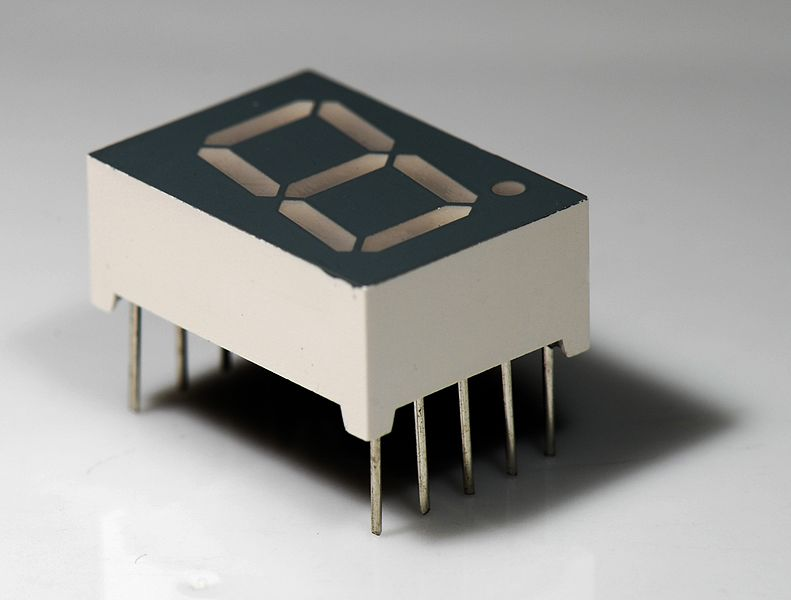
\includegraphics[width=0.25\textwidth]{figures/seven-segment-display.jpg}
	\caption{A seven segment LED display.}
	\label{fig:7-segment-display2}
\end{wrapfigure}



\subsection{Proper Interpretation of the Input Data for ICA}

When applying ICA to the handwritten digit datasets, it is interesting to note that the proper interpretation of results is not necessarily obvious.

For example, it is natural to think that the 256 pixels are the \emph{features} of our dataset and that each training example is a row. However, if we draw an analogy with the cocktail party problem, for example, and asks ourselves the questions ``What are the microphones?'' and ``What are the recordings?'', we can see that this interpretation breaks down. 

Indeed, if the training images are rows, they would correspond to the ``microphones'' of the cocktail party problem. On the other hand, the ``recordings'' would correspond to individual pixels. In other words, each ``recording'' is a vector of length 4000, containing all the values which a specific pixel takes.

This can't be useful, because each ``recording'' corresponds to a specific pixel. Hence, none of the ``recordings'' arrives from a linear combination of some sources, as all the ``recordings'' are already independent, by definition!

Therefore, we have to take the opposite viewpoint. We will treat each pixel as a ``row'' and each training example as a ``feature.'' This way, there is a ``microphone'' associated to every pixel (hence 256 ``microphones'' in total) and each training image is a ``recording.''


\subsection{ICA Reconstruction}

We are interested to know how much information is preserved and how much is lost when using ICA for the purpose of dimensionality reduction. When running the ICA algorithm with \func{n.comp = 40} sources, it also outputs the source coefficients that approximate best each image (i.e. the mixing matrix). Then, reconstructing the original training images is only a matter of multiplying the mixing matrix with the sources matrix.

\begin{figure}[H]
	\adjincludegraphics[width=0.8\textwidth, center]{figures/ica-reconstruction}
	\caption{Reconstruction of the first 10 images in each training set using the source coefficients with respect to all 40 independent components.}
	\label{fig:ica-reconstruction}
\end{figure}

The plot in Figure~\ref{fig:ica-reconstruction-gradual-digit-0} illustrates what happens to the reconstructed images as the numbers of independent components varies.

\begin{figure}[H]
	\adjincludegraphics[width=0.98\textwidth, center]{figures/ica-reconstruction-gradual-digit-zero}
	\caption{Reconstruction of the first 12 training examples for digit 0 as the number of independent components (IC) varies.}
	\label{fig:ica-reconstruction-gradual-digit-0}
\end{figure}

We observe that
\begin{enumerate}
	\item The image is almost unrecognizable for 5 independent components or less.
	\item ICA is not very good at smoothing out noise -- in fact, it seems to add noise.

\end{enumerate}

\subsection{Comparison between PCA and ICA}

At this point we would caution the reader to be careful about comparing PCA and ICA, because in this report we performed PCA on datasets of each digit \emph{seperately} and we performed ICA on a combined dataset containing all the digits \emph{together}.

As such, we restrict ourselves to generalities that would apply to any dataset. For example, we observed that the PCA components tend to overlap significantly with one another, whereas the ICA components tend not to overlap at all.

\section{PCA, ICA and Classification of Handwritten Digits}

We were interested to see how PCA and ICA could have an impact on the task of classifying handwritten digits. What would happen if we reduced the dimension of the datasets with either PCA or ICA and then applied some common classifiers? Would the performance be affected?

We carried out the experiment with four classifiers: random forests, $k$-NN, Naive Bayes and SVM. We did the experiment without data reduction, with PCA (10, 25, 50 and 100 components) data reduction and finally with ICA (10, 25, 50 and 100 components) data reduction.

% latex table generated in R 3.1.2 by xtable 1.7-4 package
% Mon Mar 16 17:56:57 2015
	\begin{table}[H]
	%\caption{Global caption}
	\begin{minipage}{.5\linewidth}
		\caption{Results of classification experiment.}
		\centering
		\begin{tabular}{lrr}
			\hline
			\textbf{\specialcell{Classification\\Method}} & \textbf{\specialcell{Accu-\\racy}} & \textbf{\specialcell{Differ-\\ence}} \\ 
			\hline
			Random Forest & $0.966$ & $0.000$ \\ 
			k-NN & $0.945$ & $0.000$ \\
			Naive Bayes & $0.745$ & $0.000$ \\
			SVM & $0.968$ & $0.000$ \\
			PCA (10) + RF & $0.899$ & $-0.067$ \\
			PCA (10) + k-NN & $0.913$ & $-0.032$ \\
			PCA (10) + NB & $0.798$ & $+0.053$ \\
			PCA (10) + SVM & $0.933$ & $-0.035$ \\
			PCA (25) + RF & $0.939$ & $-0.027$ \\
			PCA (25) + k-NN & $0.950$ & $+0.005$ \\
			PCA (25) + NB & $0.893$ & $\textbf{+0.148}$ \\
			PCA (25) + SVM & $0.968$ & $0.000$ \\
			PCA (50) + RF & $0.944$ & $-0.022$ \\
			PCA (50) + k-NN & $0.949$ & $+0.004$ \\
			PCA (50) + NB & $0.883$ & $+0.138$ \\
			PCA (50) + SVM & $0.971$ & $+0.003$ \\
			PCA (100) + RF & $0.937$ & $-0.029$ \\
			PCA (100) + k-NN & $0.952$ & $+0.007$ \\
			\hline
		\end{tabular}
	\end{minipage}%
	\qquad
	\begin{minipage}{.5\linewidth}
		\centering
		\caption{(continued) Results of classification experiment.}
		\begin{tabular}{lrr}
			\hline
			\textbf{\specialcell{Classification\\Method}} & \textbf{\specialcell{Accu-\\racy}} & \textbf{\specialcell{Differ-\\ence}} \\  
			\hline
			PCA (100) + NB & $0.877$ & $+0.132$ \\ 
			PCA (100) + SVM & $0.955$ & $-0.013$ \\ 
			ICA (10) + RF & $0.909$ & $-0.057$ \\ 
			ICA (10) + k-NN & $0.909$ & $-0.036$ \\ 
			ICA (10) + NB & $0.830$ & $+0.085$ \\ 
			ICA (10) + SVM & $0.924$ & $-0.044$ \\ 
			ICA (25) + RF & $0.944$ & $-0.022$ \\ 
			ICA (25) + k-NN & $0.940$ & $-0.005$ \\ 
			ICA (25) + NB & $0.874$ & $+0.129$ \\ 
			ICA (25) + SVM & $0.966$ & $-0.002$ \\ 
			ICA (50) + RF & $0.941$ & $-0.025$ \\ 
			ICA (50) + k-NN & $0.936$ & $-0.009$ \\ 
			ICA (50) + NB & $0.876$ & $+0.131$ \\ 
			ICA (50) + SVM & $\textbf{0.974}$ & $+0.006$ \\ 
			ICA (100) + RF & $0.941$ & $-0.025$ \\ 
			ICA (100) + k-NN & $0.930$ & $-0.015$ \\ 
			ICA (100) + NB & $0.873$ & $+0.128$ \\\ 
			ICA (100) + SVM & $0.961$ & $-0.007$ \\ 
			\hline
		\end{tabular}
	\end{minipage} 
\end{table}

The best result was obtained by applying ICA dimensionality reduction with 50 components and then using SVM. The improvement is a fairly insignificant one at $+0.006$. In fact, SVM and Random Forest both perform very well on the raw dataset and hence don't leave a lot of room for improvement.

It is interesting to note that Naive Bayes significantly benefits from both PCA and ICA, in particular when the number of components chosen is large.

All in all, the results of the experiments are inconclusive. More experiments should be conducted!

\section{Question 2: Cluster Analysis of Seeds Dataset}

In this section we analyse the UCI seeds dataset\footnote{\url{http://archive.ics.uci.edu/ml/datasets/seeds}}. This dataset has 7 real-valued features and 210 rows. Moreover, each row is labeled in category 1, 2 or 3.

First, we plotted the dataset with \func{pairs} and colorized it by class label.
\begin{figure}[htb]
	\adjincludegraphics[width=0.98\textwidth, center]{figures/seeds-pairs}
	\caption{Pairwise plots of features in the seeds dataset.}
	\label{fig:seeds-pairs}
\end{figure}

Notice from Figure~\ref{fig:seeds-pairs} that the plot of \emph{area} versus \emph{asymmetric.coefficient} seems to seperate the classes fairly well. We will therefore use this projection to illustrate the results of our clustering algorithms below.

\subsection{Clustering with $k$-means}

We ran \func{kmeans} on the seeds dataset with 3 classes and 20 iterations and obtained a first clustering. Then, we found an appropriate permutation of the labels order that matches best the true labels. We finally compared with the true labels (see Figure~\ref{fig:seeds-kmeans}) and in total 89.1\% of the entries were labeled correctly by the $k$-means clustering. 
\begin{figure}[H]
	\adjincludegraphics[width=0.98\textwidth, center]{figures/seeds-kmeans}
	\caption{$k$-means clustering of seeds dataset versus true labels.}
	\label{fig:seeds-kmeans}
\end{figure}

\subsection{Hierarchical Clustering}

We ran hierarchical clustering with the function \func{hclust} and we tried every algorithm available for the argument \func{method}. Of course, in each case the labels were assigned in an arbitrary order to the clusters, so we used the function \func{find.best.cluster.labels} (see code in Appendix)  to find a permutation of the labels ordering that matches the true labels best (i.e. we find the permutation that gives the highest classification accuracy). The results are summarized in Table~\ref{table:hclust}.
% latex table generated in R 3.1.2 by xtable 1.7-4 package
% Mon Mar 16 07:36:08 2015
\begin{table}[ht]
\centering
\begin{tabular}{lr}
  \hline
 Method & Accuracy \\ 
  \hline
 ward.D & 0.890 \\ 
 ward.D2 & 0.890 \\ 
 single & 0.371 \\ 
 complete & 0.805 \\ 
 average & \textbf{0.910} \\ 
 mcquitty & 0.762 \\ 
 median & 0.652 \\ 
 centroid & 0.557 \\ 
   \hline
\end{tabular}
\caption{Results of running \func{hclust} with different values for \func{method}}
\label{table:hclust}
\end{table}
The best results were obtained with the ``average'' method. See Figure~\ref{fig:seeds-hclust-average} for a plot of the \func{hclust} object returned by the algorithm, along with the rectangles in blue corresponding to the \func{k=3} clusters.

\begin{figure}[H]
	\adjincludegraphics[width=0.98\textwidth, center]{figures/seeds-hclust-average}
	\label{fig:seeds-hclust-average}
\end{figure}

Finally in Figure~\ref{fig:seeds-hclust-average-versus}, we see how the hierarchical clustering compares with the true labels of the data.

\begin{figure}[H]
	\adjincludegraphics[width=0.98\textwidth, center]{figures/seeds-hclust-average-versus}
	\caption{Hierarchical clustering}
	\label{fig:seeds-hclust-average-versus}
\end{figure}

\newpage

\section{Appendix}
\begin{verbatim}
# ======================================================================
# R code for Assignment #2 in STATS5703W
# Description: (1) Compute PCA and ICA on handwritten digits dataset and
# summarize the findings and (2) cluster analysis of seeds dataset.
# Written by: Philippe Paradis
# Additional credits: Part of the code was taken from Shirley
# Mills' STATS5703W course notes.
# ======================================================================
# Package requirements:
#   fastICA, caret, randomForest, parallel, lattice, e1071, xtable

# Please set the following global variables according to your system:
# 'work.dir' - Working directory in which this file is located
# 'data.dir' - Data directory containing the handwritten digit datasets
# 'code.dir' - Directory with code from STATS5703W
# 'save.to.pdf'   - Set to FALSE for interactive plotting
# 'run.parallel'  - Set to FALSE to turn off parallel computing 
# 'use.max.cores' - Maximum number of cores to use for parallel computing
#                   or 0 to use all cores available.
switch(Sys.info()[['sysname']],
Windows =
  {
     # Set the variables here if you are on Windows
     work.dir <- "D:/proj/stat5703w/ass2"
     data.dir <- "D:/proj/stat5703w/data"
     code.dir <- "D:/proj/stat5703w/code"
     save.to.pdf <- TRUE
     run.parallel <- TRUE
     use.max.cores <- 0
  },
Linux =
  {
     # Set the variables here if you are on Linux
     work.dir <- "/proj/stat5703w/ass2"
     data.dir <- "/proj/stat5703w/data"
     code.dir <- "/proj/stat5703w/code"
     save.to.pdf <- TRUE
     run.parallel <- TRUE
     use.max.cores <- 0
  },
Darwin =
  {
     # Set the variables here if you are on Mac
     work.dir <- "/proj/stat5703w/ass2"
     data.dir <- "/proj/stat5703w/data"
     code.dir <- "/proj/stat5703w/code"
     save.to.pdf <- TRUE
     run.parallel <- TRUE
     use.max.cores <- 0
  })

# Misc global variables
global.cl <- NULL

# Set 'work.amount' to "easy", "medium" or "hard" to determine
# the amount of ICA work to do. This will change the size of the
# training set fed into fastICA, which can be quite slow as the
# size of the training set increases.
work.ica.amount <- "medium"

# This sets the training/testing dataset sizes for ICA. Note that
# those are sizes *per digit*.
switch(work.ica.amount,
       easy   = {global.ica.train.size <-  80; global.ica.test.size <-  20},
       medium = {global.ica.train.size <- 200; global.ica.test.size <-  70},
       hard   = {global.ica.train.size <- 400; global.ica.test.size <- 140})

# Load required libraries
library(stats)
library(fastICA)
library(xtable)
library(randomForest)
library(class)
library(e1071)
library(caret)
library(plyr)
library(deldir)
library(combinat)

# Move to working directory and create "figures" subdirectory
# into which the plots will be saved
setwd(work.dir)
dir.create("figures", showWarnings = FALSE)

#======================================================================
# FUNCTION DEFINITIONS
#======================================================================

# This function calls 'pdf(...)' if 'save.to.pdf' is TRUE,
# otherwise it just calls 'dev.new()'
prep.out <- function(...)
{
   if (save.to.pdf)
      pdf(...)
   else
      dev.new()
}

# Source: Shirley Mills STAT5703W
plot.digits <- function(digits) {
   if (dev.cur() == 1) {
      x11(width = 6, height = 5)    # Open a graphics window of given size  
   }
   # Create a plot matrix with 144 subplots - plot in row-wise order
   layout(matrix(1:144, 12, 12, byrow = TRUE))
   # No margin (see ?par)
   oldpar <- par(mar = c(0, 0, 0, 0))
   for (i in 1:144) {
      # xaxt = "n", yaxt = "n" - no axes
      image(matrix(digits[i,],16,16)[,16:1], xaxt = "n", yaxt = "n",
            col = gray((255:0)/255))
   }
   par(oldpar)
}

# General images drawing function with variable length. It will adjust
# number of rows and columns automatically. It also accepts images of
# varying dimensions.
plot.images <- function(data, len=10, image_size=c(16,16)) {
   dim_width <- min(len, 10)
   dim_height <- ceiling(len/10)
   if (dev.cur() == 1) {
      x11(width = dim_width*8/10, height = dim_height*8/10)
   }
   # Create a plot matrix with dim_width * dim_height subplots
   layout(matrix(1:(dim_width*dim_height),
                 dim_height, dim_width, byrow = TRUE))
   # No margin (see ?par)
   oldpar <- par(mar = c(0, 0, 0, 0))
   # xaxt = "n", yaxt = "n" - no axes
   for (n in 1:len) {
      image(matrix(data[n,], image_size[1], image_size[2])[,image_size[2]:1],
            xaxt = "n", yaxt = "n",
            col = gray((255:0)/255))
   }
   par(oldpar)
}

# Function that plots a single image.
plot.image <- function(data, dim=c(16,16)) {
   if (dev.cur() == 1) {
      x11(width = 1, height = 1)
   }
   # Create a plot matrix with 144 subplots - plot in row-wise order
   layout(matrix(1:1, 1, 1, byrow = TRUE))
   # No margin (see ?par)
   oldpar <- par(mar = c(0, 0, 0, 0))
   # xaxt = "n", yaxt = "n" - no axes
   image(matrix(data, dim[1], dim[2])[,dim[2]:1], xaxt = "n", yaxt = "n",
         col = gray((255:0)/255))
   par(oldpar)
}


#####################################
# Helper function for classification
#####################################
classify <- function(pipeline, train.var, train.labels, test.var, test.labels)
{
   measures <- c()
   for (classifier in pipeline) {
      classifier.name <- classifier[[1]]
      classifier.func <- classifier[[2]]
      
      cat(paste("Fitting model '", classifier.name, "'...  ", sep=""))
      
      if (identical(classifier.func, randomForest)) {
         fit <- randomForest(train.var, train.labels,
                             xtest=test.var, ytest=test.labels,
                             ntree=200, keep.forest=TRUE)
         pred <- predict(fit, test.var)      
      } else if (identical(classifier.func, knn)) {
         fit <- knn(train.var, test.var, train.labels, k=7)
         pred <- fit
      } else {
         fit <- classifier.func(train.var, train.labels)
         pred <- predict(fit, test.var)
      }
      cm <- confusionMatrix(pred, test.labels)
      acc <- cm$overall[[1]]
      measures <- rbind(measures, list(name=classifier.name, accuracy=acc))
      cat(paste(signif(acc, 3), " accuracy\n", sep=""))
   }
   measures
}
#####################################
# Classify digits without PCA
#####################################
perf.measures <- c()

run_classifiers <- function(num_train=300, num_test=100)
{
  num.training.examples <- num_train
  num.testing.examples <- num_test
  train <- c()
  for (d in 0:9) {
    a <- 1
    b <- num.training.examples
    train <- rbind(train, cbind(d.digits[[d+1]][a:b,], d))
  }
  test <- c()
  for (d in 0:9) {
    a <- num.training.examples + 1
    b <- num.training.examples + num.testing.examples
    test <- rbind(test, cbind(d.digits[[d+1]][a:b,], d))
  }
  
  # Shuffle train and test
  set.seed(1990)
  train <- train[sample(nrow(train)),]
  test <- test[sample(nrow(test)),]
  
  # Labels
  train.labels <- as.factor(train[,257])
  train.var <- train[,-257]
  test.labels <- as.factor(test[,257])
  test.var <- test[,-257]
  
  # Fix colnames (having empty colname strings cause errors)
  colnames(train.var) <- NULL
  colnames(test.var) <- NULL
  
  pipeline <- list(c("Random Forest", randomForest),
                   c("k-NN", knn),
                   c("Naive Bayes", naiveBayes),
                   c("SVM", svm))
  classify(pipeline, train.var, train.labels, test.var, test.labels)
}

#####################################
# Classify digits after applying PCA
#####################################
# We will keep only the top 'num.pca.components' PCA components

run_classifiers_pca <- function(num.pca = 50, num_train=300, num_test=100)
{
  num.training.examples <- num_train
  num.testing.examples <- num_test
  
  train.init <- c()
  for (d in 0:9) {
    a <- 1
    b <- num.training.examples
    train.init <- rbind(train.init, cbind(d.digits[[d+1]][a:b,], d))
  }
  
  # Perform PCA on 'train.init'
  pca.train <- prcomp(train.init[, -257], center = FALSE)
  
  # Transform 'train.init'
  train.transf <- cbind(pca.train$x[ , 1:num.pca], train.init[, 257])
  
  # Load test dataset and apply PCA transform to it
  test.transf <- c()
  for (d in 0:9) {
    a <- num.training.examples + 1
    b <- num.training.examples + num.testing.examples
    prod <- d.digits[[d+1]][a:b, ] %*% pca.train$rotation[, 1:num.pca]
    test.transf <- rbind(test.transf, cbind(prod, d))
  }
  
  # Shuffle train and test
  set.seed(1990)
  train <- train.transf[sample(nrow(train.transf)), ]
  test <- test.transf[sample(nrow(test.transf)), ]
  
  # Labels
  train.labels <- as.factor(train[, num.pca+1])
  train.var <- train[, -(num.pca+1)]
  test.labels <- as.factor(test[, num.pca+1])
  test.var <- test[, -(num.pca+1)]
  
  # Fix colnames (having empty colname strings cause errors)
  colnames(train.var) <- NULL
  colnames(test.var) <- NULL
  
  str.pca <- paste("PCA (", num.pca, ")", sep="")
  pipeline <- list(c(paste(str.pca, "+ Random Forest"), randomForest),
                   c(paste(str.pca, "+ k-NN"), knn),
                   c(paste(str.pca, "+ Naive Bayes"), naiveBayes),
                   c(paste(str.pca, "+ SVM"), svm))
  classify(pipeline, train.var, train.labels, test.var, test.labels)
}

#####################################
# Classify digits after applying ICA
#####################################
# We will keep only the top 'num.pca.components' PCA components
run_classifiers_ica <- function(n.comp = 50, num_train=0, num_test=0)
{
  if (num_train > 0) {
    num.training.examples <- num_train
  } else {
    num.training.examples <- global.ica.train.size
  }
  if (num_test > 0) {
    num.testing.examples <- num_test
  } else {
    num.testing.examples <- global.ica.test.size
  }
  total <- num.training.examples + num.testing.examples
  
  # Combined all digits into one training dataset
  combined <- c()
  for (d in 0:9) {
    a <- 1
    b <- total
    combined <- rbind(combined, d.digits[[d+1]][a:b,])
  }
  
  set.seed(0) #for reproducibility
  w.init <- matrix(rnorm(n.comp*n.comp), n.comp, n.comp)
  t1 <- proc.time()
  # Perform ICA on 'combined' (includes all digits, as well
  # as trainin set and testing set)
  ica.train <- fastICA(t(combined),
                       n.comp,
                       alg.typ = "parallel",
                       fun = "logcosh",
                       alpha = 1,
                       method = "R",
                       row.norm = FALSE,
                       maxit = 200,
                       tol = 0.0001,
                       verbose = TRUE,
                       w.init=w.init)
  cat(paste("fastICA (n.comp = ", n.comp, ") elapsed time: ",
            (proc.time()-t1)[["elapsed"]], " seconds\n", sep=""))
  
  train.transf <- c()
  for (d in 0:9) {
    a <- 1 + d*total
    b <- num.training.examples + d*total
    train.transf <- rbind(train.transf, cbind(t(ica.train$A)[a:b,], d))
  }
  
  test.transf <- c()
  for (d in 0:9) {
    a <- num.training.examples + 1 + d*total
    b <- num.training.examples + num.testing.examples + d*total
    test.transf <- rbind(test.transf, cbind(t(ica.train$A)[a:b,], d))
  }
  
  # Shuffle train and test
  set.seed(1990)
  train <- train.transf[sample(nrow(train.transf)), ]
  test <- test.transf[sample(nrow(test.transf)), ]
  
  # Labels
  train.labels <- as.factor(train[, n.comp+1])
  train.var <- train[, -(n.comp+1)]
  test.labels <- as.factor(test[, n.comp+1])
  test.var <- test[, -(n.comp+1)]
  
  # Fix colnames (having empty colname strings cause errors)
  colnames(train.var) <- NULL
  colnames(test.var) <- NULL
  
  str.ica <- paste("ICA (", n.comp, ")", sep="")
  pipeline <- list(c(paste(str.ica, "+ Random Forest"), randomForest),
                   c(paste(str.ica, "+ k-NN"), knn),
                   c(paste(str.ica, "+ Naive Bayes"), naiveBayes),
                   c(paste(str.ica, "+ SVM"), svm))
  classify(pipeline, train.var, train.labels, test.var, test.labels)
}


#################################################################
# Although it's not necessarily to do an explicit clean up, the
# parallel workers can be shutdown by calling this function.
#################################################################
clean_parallel_env <- function()
{
   if (!is.null(global.cl))
      tryCatch(stopCluster(global.cl), error=function(e) FALSE)
   global.cl <<- NULL
}

##############################################################
# Setup parallel environment (if 'run.parallel' is TRUE) and
# if more than 1 core was detected.
##############################################################
setup_parallel_env <- function()
{
   if (!run.parallel)
      return(NULL)
   
   library(parallel)
   avail.cores <- detectCores()
   cat(paste("Detected ", avail.cores, " cores...\n", sep=""))
   if (avail.cores <= 1) {
      run.parallel <- FALSE
      global.cl <<- NULL
   } else {
      if (use.max.cores > 0) {
         num.cores <- min(avail.cores, use.max.cores)
         cat(paste("Launching ", num.cores,
                   " worker threads in parallel...\n", sep=""))
      } else {
         num.cores <- avail.cores
      }
      clean_parallel_env()
      cl <- makePSOCKcluster(num.cores, outfile="",
                             useXDR=FALSE)
      #setDefaultCluster(cl)
      # Export the necessary variables and functions
      clusterExport(cl, c("d.digits", "combined.d.digits", "randomForest",
                          "global.ica.train.size", "global.ica.test.size",
                          "run_classifiers_pca", "run_classifiers_ica",
                          "knn", "naiveBayes", "svm",
                          "classify", "confusionMatrix", "fastICA"))
      global.cl <<- cl
   }
}

#################################################################
# This function returns FALSE if at least one of the connections
# to the workers was shut down, otherwise it returns TRUE.
#################################################################
check_parallel_connections <- function()
{
   tryCatch(all(sapply(sapply(global.cl, "[")["con",], isOpen)),
            error=function(e) FALSE)
}

##################################################################
# Just call this like 'lapply'. Parallelism will be automatically
# handled by this function, including initialization/cleanup of
# worker threads. The function will proceed sequentially if
# parallelismm is disabled or if the system is single core.
##################################################################
parallel_lapply <- function(X, FUN)
{
   if (run.parallel) {
      # Check if 'global.cl' was defined
      if (is.null(global.cl))
         setup_parallel_env()
      # Check if the connections in 'global.cl' were closed down
      else if (!check_parallel_connections())
         setup_parallel_env()
      if (!is.null(global.cl)) {
         cat(paste("Running ", length(X)," tasks in parallel...\n", sep=""))
         flush.console()
         results <- tryCatch(parLapplyLB(global.cl, X, FUN),
                             error=function(e){clean_parallel_env(); stop(e)})
         return(results)
      }
   }
   return(lapply(X, FUN))
}

#######################################################
# Load handwritten digits training datasets
#######################################################
d.file <- {}
d.digits <- c({}, {}, {})
for (i in 0:9) {
   d.file[i+1] <- paste(data.dir, "/train_", i, ".dat", sep = "")
   d.digits[[i+1]] <- matrix(scan(d.file[i+1], sep = ","),
                             ncol = 256, byrow = T)
}

#######################################################
# Perform PCA
#######################################################
# Perform PCA analysis on each training set independently
# i.e. on each digit independently
pc.digits <- {}
prep.out("figures/digits-pca.pdf", height=4)
par(mfrow=c(2,5), mar=c(4.1,2.1, 2.1, 1.1))
for (i in 0:9) {
   # Important: 'center' is set to FALSE. This makes analysis
   # much simpler, especially since our data is already fairly well
   # centered.
   pc.digits[[i+1]] <- prcomp(d.digits[[i+1]], center = FALSE)
   plot(pc.digits[[i+1]], col = heat.colors(10), main = i)
   
   # Uncomment the following to see a summary of the PCA results...
   # print(summary(pc.digits[[i+1]]))
}
dev.off()

#######################################################
# Calculate cumulative proportion of variance explained
#######################################################

# This function computes how many top PCA components are
# necessary to explain a variance of at least 'min.variance'
how.many.pcs.for.variance <- function (min.variance)
{
   results <- matrix(NA, 2, 10)
   for (i in 0:9) {
      for (pc.index in 1:256) {
         cumul <- sum(pc.digits[[i+1]]$sdev[1:pc.index]^2) /
            sum(pc.digits[[i+1]]$sdev^2)
         if (cumul >= min.variance) {
            results[,i+1] <- c(i, pc.index)
            break
         }
      }
   }
   
   for (i in 0:9) {
      print(paste("The first", results[2,i+1],
                  "principal components of the digit",
                  i, "explain", cumul, "% of the total variance."))
   }
   results
}

# Call the above function
(req.pcs <- how.many.pcs.for.variance(0.95))

# Produce LaTeX table describing this result
row.names(req.pcs) <- c("Digit", "# of Components")
xres <- xtable(req.pcs)
print(xres, include.colnames = FALSE)

####################################################
# Examine the PCA components one by one and
# investigate what abstract 'features' they measure
####################################################

num_pcs <- 256
pc <- array(dim = c(num_pcs, 256, 10),
            dimnames = list(c(1:num_pcs),1:256,c(0:9)))
for (j in 1:num_pcs) {
   for (i in 0:9) {
      pc[j,,i+1] <- pc.digits[[i+1]]$rotation[,j]
   }
}

# Source: Shirley Mills STAT5703W
display.mean.pc <- function(pca_comp, digits) {
   mean <- apply(digits, 2, mean)
   for (i in 1:15) {
      image(matrix(mean+(i-8)*pca_comp, 16,16)[,16:1],
            xaxt = "n", yaxt = "n", col = gray((255:0)/255))
   }
}

# Source: Shirley Mills STAT5703W
display.pcs <- function (pcnum) {
   if (dev.cur() == 1) {
      x11(width = 7, height = 5)
   }
   oldpar <- par(mar = c(0, 0, 0, 0))
   layout(matrix(1:150, 10, 15, byrow = TRUE))
   for (i in 0:9) {
      display.mean.pc(pc[pcnum,,i+1], d.digits[[i+1]])
   }
   par(oldpar)
}

prep.out("figures/top-pcs-digit-0.pdf", height=3)
plot.images(t(pc.digits[[0+1]]$rotation), 40)
dev.off()

prep.out("figures/pc-1.pdf", width=7, height=5)
display.pcs(1)
dev.off()

prep.out("figures/pc-2.pdf", width=7, height=5)
display.pcs(2)
dev.off()

#####################################
# Reconstruction of digits with PCA
#####################################
d.digits.pc <- {}
for (i in 0:9) {
   d.digits.pc[[i+1]] <- d.digits[[i+1]]%*%pc.digits[[i+1]]$rotation
}

num.cases <- unlist(lapply(d.digits, dim))[seq(1,20,2)]
num.features <- unlist(lapply(d.digits, dim))[seq(2,21,2)]
num.table <- xtable(rbind(num.cases, num.features))
row.names(num.table) <- c("Training Examples", "Features")
print(num.table)

# Recreate a digit from some subset of its PCA coefficients
recreate <- function(pc.range, digit) {
   tmp <- matrix(0, num.cases[digit+1], 256)
   tmp <- d.digits.pc[[digit+1]][,pc.range] %*%
      t(pc.digits[[digit+1]]$rotation[,pc.range])
   tmp <- tmp/max(abs(range(tmp))) # Scale the data to lie in [-1, 1]
   tmp
}

# Recreate a digit from some subset of its PCA coefficients
# Also, add center and rescale as necessary
recreate.clean <- function(pc.range, digit) {
   tmp <- matrix(0, num.cases[digit+1], 256)
   tmp <- d.digits.pc[[digit+1]][,pc.range] %*% 
      t(pc.digits[[digit+1]]$rotation[,pc.range])
   #Add the center and rescale back data
   if (!identical(pc.digits[[digit+1]]$scale, FALSE)) {
      tmp <- scale(tmp, center = FALSE , scale=1/pc.digits[[digit+1]]$scale)
   }
   if (!identical(pc.digits[[digit+1]]$center, FALSE)) {
      # For presentation purposes, we introduce 'clean.coeff', which
      # takes care of cleaning 
      clean.coeff <- (256-max(pc.range))/256*-1*pc.digits[[digit+1]]$center
      tmp <- scale(tmp, center = clean.coeff, scale=FALSE)
   }
   tmp <- tmp/max(abs(range(tmp))) # Dcale the data to lie in [-1, 1]
   tmp
}

# Recreate training sets digits using the PCs specified by 'pc.range'
plot.recreate.all <- function(pc.range) {
   if (dev.cur() == 1) {
      x11(width = 8, height = 8/12*10) 
   }
   # Create a plot matrix with 144 subplots - plot in row-wise order
   layout(matrix(1:120, 10, 12, byrow = TRUE))
   # No margin (see ?par)
   oldpar <- par(mar = c(0, 0, 0, 0))
   for (d in 0:9) {
      recreated.digits <- recreate(pc.range, d)
      for (i in 1:12) {
         # xaxt = "n", yaxt = "n" - no axes
         image(matrix(recreated.digits[i,],16,16)[,16:1],
               xaxt = "n", yaxt = "n", col = gray((255:0)/255))
      }
   }
   par(oldpar)
}

# Recreate training sets digits using the PCs specified by 'pc.range'
plot.recreate.gradual <- function(digit) {
   if (dev.cur() == 1) {
      x11(width = 9, height = 8/12*10) 
   }
   # Create a plot matrix with 144 subplots - plot in row-wise order
   layout(matrix(1:130, 10, 13, byrow = TRUE))
   # No margin (see ?par)
   oldpar <- par(mar = c(0, 0, 0, 0))
   plot.new()
   text(0.5, 0.5, labels="Origi-\nnal", cex=2)
   for (i in 1:12) {
      image(matrix(d.digits[[digit+1]][i,],16,16)[,16:1],
            xaxt="n", yaxt="n", col = gray((255:0)/255))
   }
   for (num.pcs in c(1,2,3,5,15,30,75,150,256)) {
      pc.range <- 1:num.pcs
      recreated.digits <- recreate.clean(pc.range, digit)
      plot.new()
      text(0.5, 0.5, paste(num.pcs, "\nPCs"), cex=2)
      for (i in 1:12) {
         # xaxt = "n", yaxt = "n" - no axes
         image(matrix(recreated.digits[i,],16,16)[,16:1], 
               xaxt = "n", yaxt = "n", col = gray((255:0)/255))
      }
   }
   par(oldpar)
}

prep.out("figures/recreate-gradual-digit-0.pdf", width=9, height=7)
plot.recreate.gradual(0)
dev.off()

#######################################
# Perform ICA on the combined datasets
#######################################

# Combine the training datasets for digits 0 to 9 into
# a single matrix called 'combined.d.digits'.
# Because the size of the training sets for the various digits is
# not the same, we only take the first 'num.training.examples' rows 
# for each digit, in order to keep the dataset balanced.

num.training.examples <- global.ica.train.size
combined.d.digits <- c()
for (d in 0:9) {
   combined.d.digits <- rbind(combined.d.digits,
                              d.digits[[d+1]][1:num.training.examples,])
}

n.comp <- 40

set.seed(0) #for reproducibility
w.init <- matrix(rnorm(n.comp*n.comp), n.comp, n.comp)

t1 <- proc.time()
combined.ica.digits <- fastICA(t(combined.d.digits),
                               n.comp,
                               alg.typ = "parallel",
                               fun = "logcosh",
                               alpha = 1,
                               method = "R",
                               row.norm = FALSE,
                               maxit = 200,
                               tol = 0.0001,
                               verbose = FALSE,
                               w.init = w.init)
cat(paste("fastICA (n.comp = ", n.comp, ") elapsed time: ",
          (proc.time()-t1)[["elapsed"]], " seconds\n", sep=""))
# Plot all the ICA components
prep.out("figures/ica-components.pdf", width=8, height=4)
plot.images(t(combined.ica.digits$S), n.comp)
dev.off()

########################################################################
# Reconstruct first 10 examples from training sets for each digit
########################################################################
index.first.twelve <- rep(1:10, 10) + rep(seq(0, 9*num.training.examples,
                                              num.training.examples), each=10)

prep.out("figures/ica-reconstruction.pdf", width=8, height=8)
plot.images(t(combined.ica.digits$S %*%
                 combined.ica.digits$A)[index.first.twelve, ],
            length(index.first.twelve))
dev.off()

########################################################################
# Reconstruction of digit 0 for different number of ICA components
########################################################################
fast.reconstruct.zero <- function(n.comp)
{
   set.seed(1990) # for reproducibility
   w.init <- matrix(rnorm(n.comp*n.comp), n.comp, n.comp)
   t1 <- proc.time()
   ica <- fastICA(t(combined.d.digits),
                  n.comp,
                  alg.typ = "parallel",
                  fun = "logcosh",
                  alpha = 1,
                  method = "R",
                  row.norm = FALSE,
                  maxit = 200,
                  tol = 0.0001,
                  verbose = TRUE,
                  w.init = w.init)
   cat(paste("fastICA (n.comp = ", n.comp, ") elapsed time: ",
             (proc.time()-t1)[["elapsed"]], " seconds\n", sep=""))
   ica
}

n.comp.list <- c(1,2,3,5,15,30,75,150,255)
ica.list <- parallel_lapply(n.comp.list, fast.reconstruct.zero)

# Reconstruct the first 12 digits in the training set for each ICA soln
images.reconstructed.list <- c()
for (ica in ica.list) {
   images.reconstructed.list <- rbind(images.reconstructed.list,
                                      list(t(ica$S %*% ica$A)[1:12, ]))
}

prep.out("figures/ica-reconstruction-gradual-digit-zero.pdf", width=9, height=7)
if (dev.cur() == 1) {
   x11(width = 9, height = 8/12*10) 
}
# Create a plot matrix with 144 subplots - plot in row-wise order
layout(matrix(1:130, 10, 13, byrow = TRUE))
# No margin (see ?par)
oldpar <- par(mar = c(0, 0, 0, 0))
plot.new()
text(0.5, 0.5, labels="Origi-\nnal", cex=2)
# Plot original digit 0
for (i in 1:12) {
   image(matrix(d.digits[[0+1]][i,],16,16)[,16:1],
         xaxt="n", yaxt="n", col = gray((255:0)/255))
}
# Here we use apply to simultaneously loop over the two
# lists 'n.comp.list' and 'img.rows.list'
apply(data.frame(n.comp.list, images.reconstructed.list, length(n.comp.list)),
      1,
      function(pair) {
         n.comp <- pair[[1]]
         img <- pair[[2]]
         
         plot.new()
         text(0.5, 0.5, paste(n.comp, "\nICs"), cex=2)
         for (i in 1:12) {
            # xaxt = "n", yaxt = "n" - no axes
            image(matrix(img[i,],16,16)[,16:1], 
                  xaxt = "n", yaxt = "n", col = gray((255:0)/255))
         }
      })
par(oldpar)
dev.off()


prep.out("figures/ica-recreate-gradual-digit-0.pdf", width=9, height=7)
plot.recreate.gradual(0)
dev.off()

###########################################################
# Helper function for running parallel jobs
###########################################################
run_job <- function(job)
{
   type <- job[[1]]
   n.comp <- job[[2]]
   
   if (type == "pca")
      return(run_classifiers_pca(n.comp))
   else if (type == "ica")
      return(run_classifiers_ica(n.comp))
   stop(simpleError("Invalid job type submitted."))
}

###########################################################
# Run classification tasks
###########################################################
m <- run_classifiers()
# Launch the jobs in parallel

A <- c("pca", "ica")
B <- c(10, 25, 50, 100)
# Build the cartesian product A x B
jobs.list <- dlply(expand.grid(A, B), 1:2, c)
# Run the jobs
m_jobs <- parallel_lapply(jobs.list, run_job)

# Show the results :)
perf.measures <- do.call(rbind, c(list(m), m_jobs))
xres <- xtable(perf.measures[order(unlist(perf.measures[,"accuracy"]),
                                   decreasing=TRUE),], digits=3)
print(xres, include.rownames = FALSE)

# Show results with deltas! :)
M <- perf.measures
num.A <- length(A)
num.B <- length(B)
num.C <- 4 # Number of classifiers used
M <- cbind(M, rep(0, num.C))
for (a in 1:num.A) {
   for (b in 1:num.B) {
      s <- seq(num.C+b+(num.C*num.B)*(a-1),
               num.C+num.C*num.B+(num.C*num.B)*(a-1),
               num.C)
      M[s,3] <- unlist(M[s,2]) - rep(M[[b,2]], num.C)
   }
}
xres <- xtable(M, digits=3)
print(xres, include.rownames = FALSE)


############################################################
# QUESTION 2: Clustering of seeds dataset
############################################################


############################################################
# Load and format seeds dataset
############################################################
seeds <- read.table("seeds_dataset.txt", header=FALSE,
                    colClasses = c(rep("numeric", 7),
                                   "factor"),
                    col.names=c("area", # area A,
                                "perimeter", # perimeter P,
                                "compactness", # compactness C 
                                "kernel.length", # length of kernel, 
                                "kernel.width", # width of kernel, 
                                "asymmetric.coefficient",
                                "kernel.groove.length",
                                "class" # {karma, rosa, canadian}
                    ))

seeds.class <- as.numeric(seeds$class)

#########################################################################
# This function generates all permutations of the labels and applies
# it to 'cluster'. It compares it with the actual labels and returns the
# cluster with the labels permutation having the lowest error rate.
#########################################################################
find.best.cluster.labels <- function(cluster, actual, num.labels)
{
   best_acc <- 0
   best_cluster <- c()
   permutations <- permn(num.labels)
   for (p in permutations) {
      new_cluster <- cluster
      c <- 1
      for (x in p) {
         new_cluster[cluster==c] <- x
         c <- c+1
      }
      acc <- sum(new_cluster == actual)
      if (acc > best_acc) {
         best_acc <- acc
         best_cluster <- new_cluster
      }
   }
   best_cluster
}

############################################################
# Plot elementary graphs about seed
############################################################
run_hierarchical_clustering <- function(seeds, seeds.class)
{
   # Hierarchical clustering   
   methods = c("ward.D", "ward.D2", "single", "complete", "average",
               "mcquitty", "median", "centroid")
   classes.clust.avg <- c()
   
   seeds.dist <- dist(seeds[,-8])
   
   results <- c()
   for (method in methods) {
      seeds.hclust <- hclust(seeds.dist, method=method)
      seeds.hclust$labels <- seeds$class
      pdf(paste("figures/seeds-hclust-", method, ".pdf", sep=""),
          width=8, height=6)
      oldpar <- par(mar=c(5,4,1,1))
      # Produce hierarchical clustering graph
      plot(seeds.hclust, 
           main=paste("Hierarchical clustering with method '",
                      method, "'", sep=""))
      # Split into 3 clusters and label with blue rectangles
      in.clust <- rect.hclust(seeds.hclust, k=3, border="blue")
      par(oldpar)
      dev.off()
      
      # Compute the clustering accuracy
      classes.clust <- c()
      classes.clust[unname(in.clust[[1]])] <- 1
      classes.clust[unname(in.clust[[2]])] <- 2
      classes.clust[unname(in.clust[[3]])] <- 3
      
      # Find correct labels permutation
      correct.classes.clust <- find.best.cluster.labels(classes.clust,
                                                        seeds.class, 3)
      
      # Add results to 'results' table
      cm <- confusionMatrix(seeds$class, correct.classes.clust)
      acc <- cm$overall[[1]]
      results <- rbind(results, list(method, acc))
      
      # Save the results from method "average" for later
      if (method == "average")
         classes.clust.avg <- classes.clust
   }
   colnames(results) <- c("Method", "Accuracy")
   print(xtable(results, digits=3))
   
   pdf("figures/seeds-hclust-average-versus.pdf", width=8, height=4)
   oldpar <- par(mfrow=c(1,2), mar=c(5,2.5,2,1))
   plot(area ~ asymmetric.coefficient, seeds, col=classes.clust.avg, pch=17,
        main="Hierachical clustering using 'average'")
   plot(area ~ asymmetric.coefficient, seeds, col=seeds.class, pch=17,
        main="Actual labels")
   par(oldpar)
   dev.off()
}

########################################################
# Run vector quantization (k-means) on seeds dataset
########################################################
run_vector_quantization_clustering <- function(seeds, seeds.class)
{
   # Produce colorized pairs-plot
   pdf("figures/seeds-pairs.pdf", width=8, height=8)
   pairs(seeds[,1:7], col = seeds.class+1, cex.labels=1.0)
   dev.off()
   
   # Compute k-means
   set.seed(1990)
   (seeds.kmeans <- kmeans(seeds[,-8], 3, 20, algorithm="Hart"))
   correct.cluster <- find.best.cluster.labels(seeds.kmeans$cluster,
                                               seeds.class, 3)
   cm <- confusionMatrix(correct.cluster, seeds[,8])
   acc <- cm$overall[[1]]
   
   print(cm$table)
   print(paste("Accuracy:", signif(acc, 4)))
   
   pdf("figures/seeds-kmeans.pdf", width=8, height=4)
   oldpar <- par(mfrow=c(1,2), mar=c(5,2.5,2,1))
   plot(area ~ asymmetric.coefficient, seeds, col=correct.cluster, pch=17,
        main="k-means clustering")
   plot(area ~ asymmetric.coefficient, seeds, col=seeds.class, pch=17,
        main="Actual labels")
   par(oldpar)
   dev.off()
}

run_vector_quantization_clustering(seeds, seeds.class)
run_hierarchical_clustering(seeds, seeds.class)
\end{verbatim}

%\bibliographystyle{abbrv}
%\bibliography{report1}

%\clearpage
%\clearpage
\end{document}
